
% relevanzwerte und priorität erklären (nicht erklären dass die von
%0-100 gehn und prozente darstellen das erfolgt in schnittstellen)

Dieses Kapitel befasst sich mit den essenziellen Vorbetrachtungen zur
Projektarbeit. Dabei geht es vorrangig um {\"U}berlegungen zur Fehlererkennung
und der Handhabung von Verbindungsabbr{\"u}chen bzw. fehlerhaften
{\"U}bertragungen. In diesem Kontext werden die Notwendigkeit einer TTL sowie
die unterschiedlichen Optionen zur Realisierung einer Datenkonsistenzpr{u}fung
via CRC-Checksumme er{\"o}rtert. Desweiteren werden {\"U}berlegungen
bez{\"u}glich der Entwicklung des CROP Protokollstacks aufgezeigt und analysiert.

\textbf{Time To Live}

Die TTL bezeichnet die Lebensdauer eines Datenpakets und ist dabei von
unterschiedlichen Aspekten abh{\"a}ngig. So kann ein Paket einerseits nach
Ablauf eines Zeitraums verworfen werden oder aber nach einer bestimmten Anzahl
von hops. Das Ablaufen durch den hop count ist dabei in einem Szenario
interplanetarer Kommunikation derzeit eher unrealistisch, da zumei{\ss}t eine
point-to-point verbindung anvisiert wird (kein intensives Routing {\"u}ber eine
Vielzahl an Stationen). Somit w{\"a}re unter Ber{\"u}cksichtigung einer
Interplanetare Kommunikation eher eine TTL Realisierung per Zeitstempel
sinnvoll, da hier{\"u}ber unrealistische {\"U}bertragungszeiten einfach erkannt
werden k{\"o}nnen (unter Ber{\"u}cksichtigung des {\"U}bertragungskontextes).
\todo{wir hatten glaub ich schon ein erstes konzept/ideen zur umsetzung}

\textbf{Protocol Stack}

\begin{figure}[H]
\centering
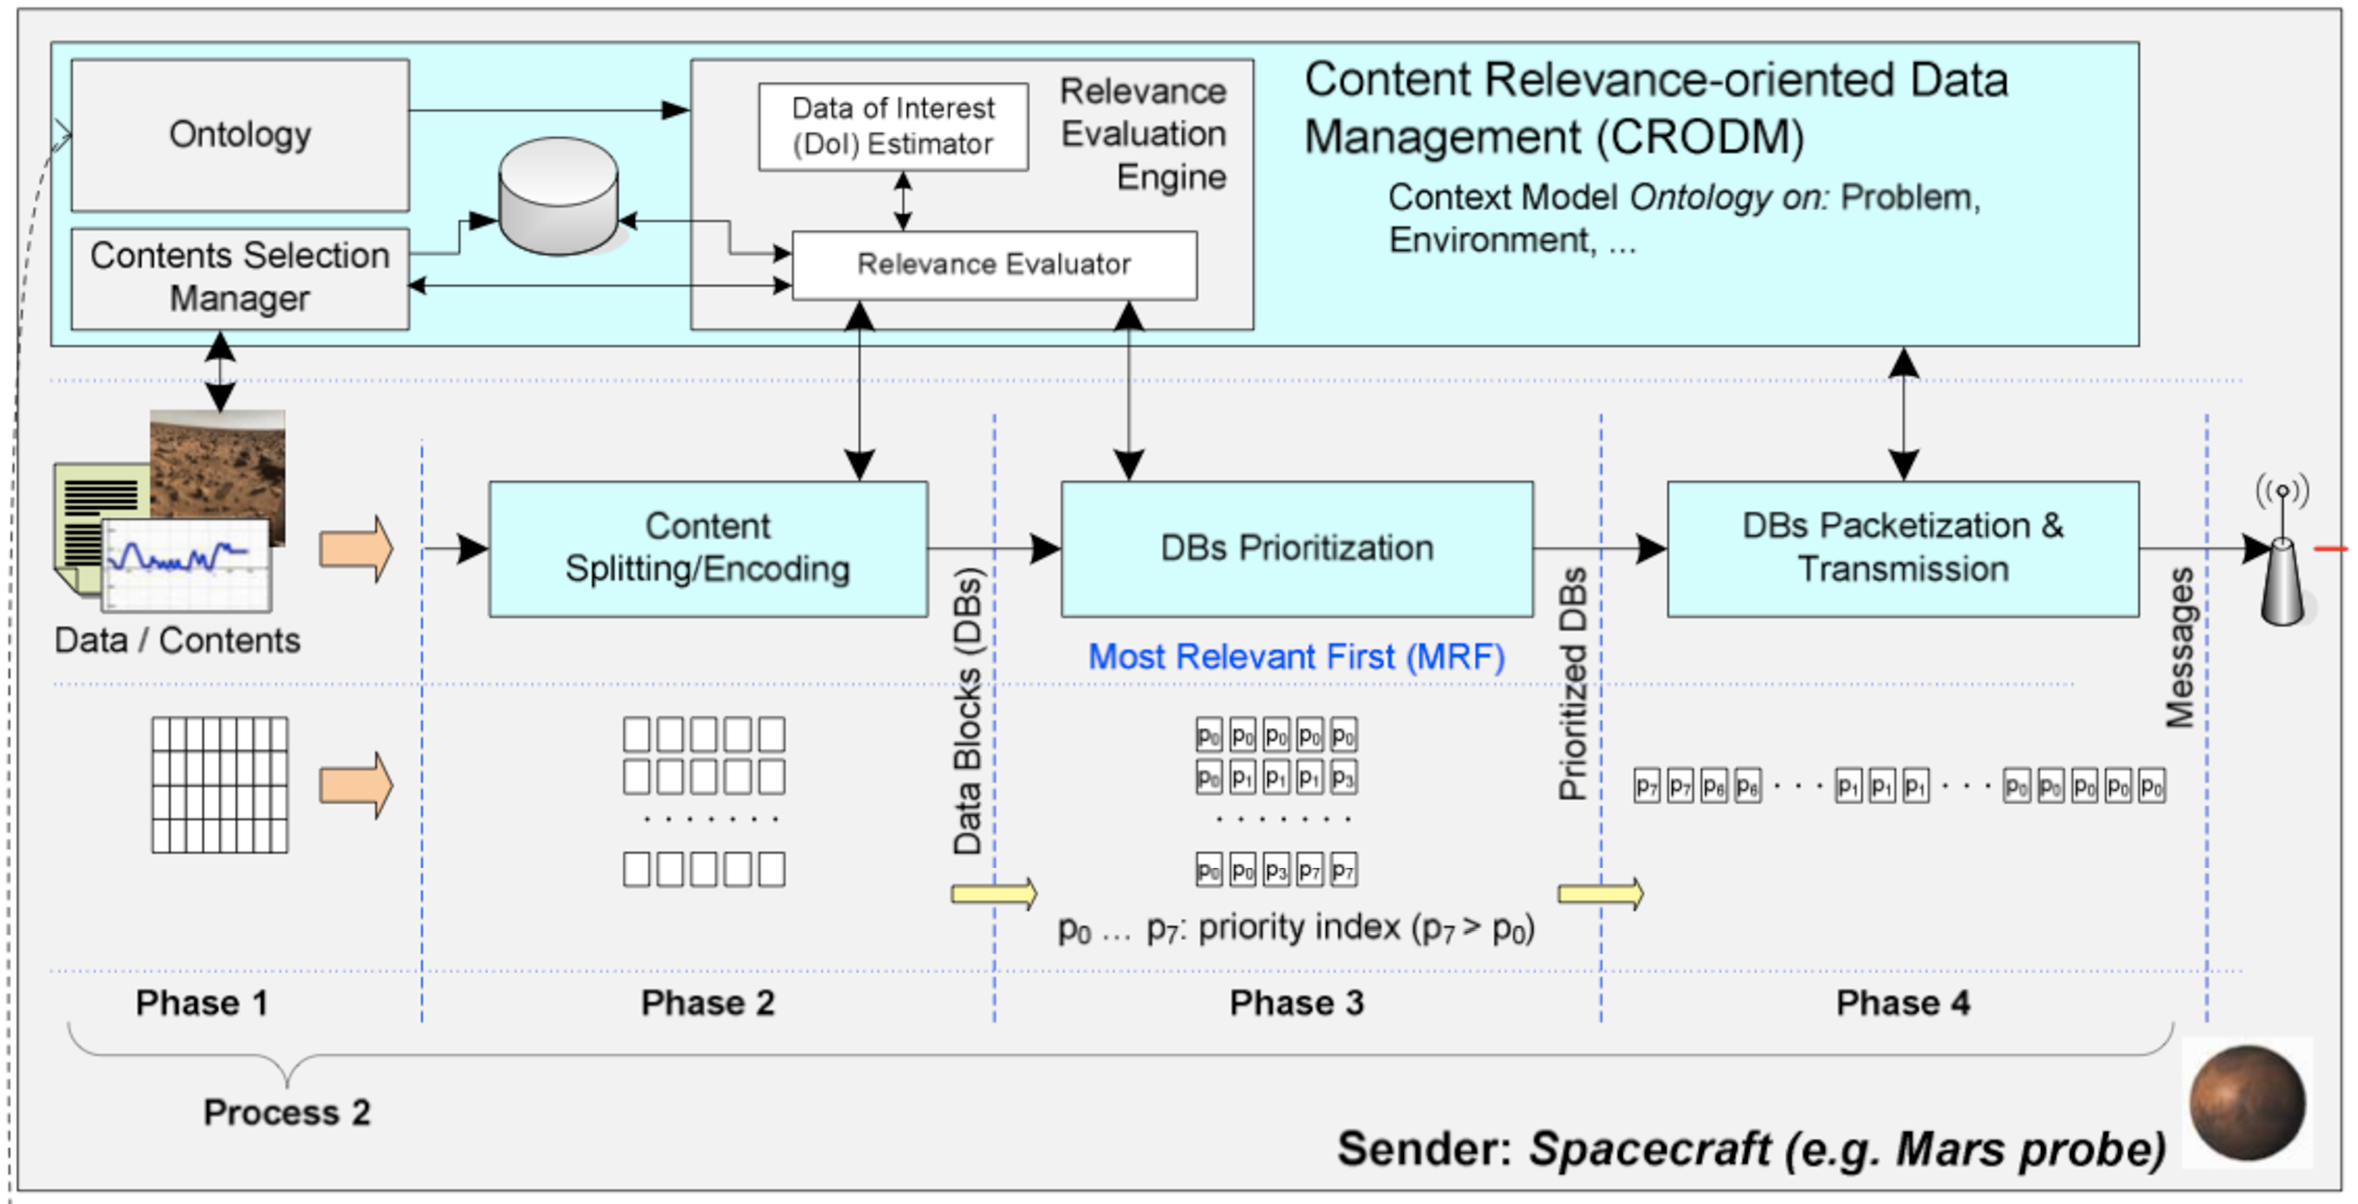
\includegraphics[scale=.25]{CRODT.pdf}
\caption{Das CRODT Framework}
\label{fig:CRODT}
\end{figure}

\textbf{Error Correction Code}

Zur Fehlererkennung bzw. Korrektur kommt ein CRC-Code zum Einsatz. Dieser kann
innerhalb des Protokolls je nach Paketgr{\"o}{\ss}e auf CRC 16 Bit oder CRC 32
Bit eingestellt werden. Die Pr{\"u}fsumme wird durch einen mathematischen
Algorithmus ermittelt und dann mit dem Paket {\"u}bertragen. Wenn der
Empf{\"a}nger die R{\"u}ckrechnung unter Einbeziehnung der Pr{\"u}fsumme
vornimmt, kann anhand des Ergebnisses ermittelt werden ob das Paket
verf{\"a}lscht wurde. Die Berechnung einer Checksumme funktioniert dabei wie
folgt:

Das zu {\"u}bertragende Datenframe sei exemplarisch gegeben als: 11 0101 1011.
Desweiteren wird ein CRC-Generatorpolynom ben{\"o}tigt, welches im Beispiel als
$G(x) = x^4 + x + 1$ gegeben sei. Die daraus resultierende Schreibweise in Generatorbits lautet: 10011
($1*x^4+0*x^3+0*x^2+1*x^1+1*x^0$).
Nun wird eine erweiterte Darstellung des zu {\"u}bertragenden Frames erzeugt,
woraus der folgende Ausdruck hervorgeht: 11 0101 1011 0000
(Frame-0-Bits; Erweiterung des Datenframes um die Ordnung des Generatorpolynoms in Nullen). Nun erfolgt eine
Division des erweiterten Frames durch das Generatorpolynom.

\makeatletter
\def\cline#1{\noalign{\vskip-2ex}\@cline#1\@nil}
\makeatother

\begin{figure}[H]
\jot-0.6mm
\begin{alignat*}{14}
1&1&0&1&0&1&1&0&1&1&0&0&0&0& : 10011=1100001010 \\
1&0&0&1&1\\ \cline{1-5}
&1&0&0&1&1& \\ 
&1&0&0&1&1& \\ \cline{2-6}
&&0&0&0&0&1& \\ 
&&1&0&0&1&1& \\ \cline{3-7}
&&&0&0&0&1&0& \\                                                 
&&&1&0&0&1&1& \\ \cline{4-8}
&&&&0&0&1&0&1& \\                                               
&&&&1&0&0&1&1& \\ \cline{5-9}
&&&&&0&1&0&1&1& \\                                           
&&&&&1&0&0&1&1&  \\ \cline{6-10}                                                                                  
&&&&&&1&0&1&1&0& \\                                           
&&&&&&1&0&0&1&1& \\   \cline{7-11}                                                                                      
&&&&&&&0&1&0&1&0& \\                                         
&&&&&&&1&0&0&1&1& \\ \cline{8-12}                                                                                     
&&&&&&&&1&0&1&0&0& \\                                       
&&&&&&&&1&0&0&1&1& \\ \cline{9-13}                                                                               
&&&&&&&&&0&1&1&1&0& \\                                     
&&&&&&&&&1&0&0&1&1& \\ \cline{10-14}    
&&&&&&&&&&1&1&1&0& 
\end{alignat*}
\end{figure}

Das Ergebnis dieser Division (der Rest in Zahlen: 1110) wird an das
urspr{\"u}nglich zu {\"u}bertragende Frame (11 0101 1011) angeh{\"a}ngt. Somit ergibt sich
nun das Frame inklusive Pr{\"u}fsumme: 11 0101 1011 1110. Der
Empf{\"a}nger kann nun {\"u}berpr{\"u}fen, ob der Frame korrekt {\"u}bertragen
wurde, indem er durch das Generatorpolynom (Generatorbits) teilt. Das Ergebnis
muss dabei 0 sein. Das im Beispiel genutzte Polynom kann mit der Ordnung 4
($2^4=16$) auf 16 Bits an Daten angewandt werden. Das Polynom $x16+x12+x5+1$
wird hingegen beispielsweise beim CRC-CCITT 16 Bit verfahren genutzt und
kann auf Datenframes bis zu einer Gr{\"o}{\ss}e von $2^{16}=65536 Bit$
angewendet werden (Polynom eines 32 Bit CRC entsrechend mit Ordnung 32).

